% =============================================================================
% Seção 3 — Arquitetura do Sistema
% =============================================================================

\section{Arquitetura do Sistema}
\label{sec:arquitetura}

O NeuroAssist AI é composto por dois contextos implantáveis: um \emph{pipeline de
detecção no navegador}, executado inteiramente no dispositivo do paciente, e um
\emph{pipeline de alertas no backend}, implementado como microsserviços hexagonais.
A Figura~\ref{fig:visaogeral} ilustra o fluxo de dados ponta-a-ponta.

\subsection{Visão Geral do Sistema}
\label{sec:visaogeral}

O pipeline é acionado por um gesto facial deliberado capturado por qualquer webcam
comum (720\,p ou superior). O loop de detecção de gestos é executado exclusivamente
no navegador via WebAssembly; nenhum quadro de vídeo sai do dispositivo em nenhum
momento. Quando um gesto é confirmado pela máquina de estados
(Seção~\ref{sec:maquinadeestados}), um payload JSON leve é enviado via POST ao serviço
de ingestão de eventos. O serviço valida o gesto contra o perfil de detecção ativo do
paciente, cria um registro \texttt{Evento} e despacha uma notificação
\texttt{FULL\_SCREEN\_ALARM}. A aplicação do cuidador consulta o backend a cada cinco
segundos; ao detectar um evento ativo, renderiza uma sobreposição de alarme em tela
cheia. O cuidador confirma o atendimento, o que grava um \texttt{verdict} de volta ao
registro do evento e limpa o alarme.

\begin{figure*}[!t]
  \centering
  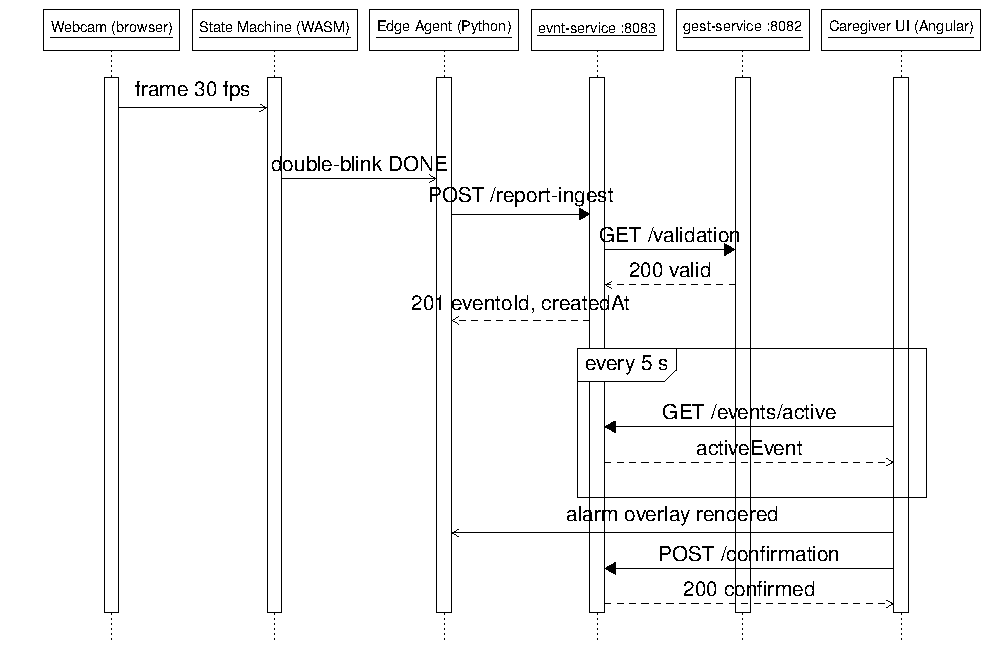
\includegraphics[width=\textwidth]{../template/figures/fig_overview}
  \caption{Fluxo de dados ponta-a-ponta. O vídeo é processado inteiramente no
    navegador (WASM); apenas relatórios JSON estruturados cruzam a fronteira de rede.}
  \label{fig:visaogeral}
\end{figure*}

\subsection{Detecção de Gesto Offline-First}
\label{sec:deteccao}

A extração de marcos faciais é realizada pelo MediaPipe
FaceLandmarker~\cite{lugaresi2019mediapipe} executando no delegate WebAssembly de CPU.
O binário WASM e o modelo de marcos faciais \texttt{float16} são empacotados como
ativos estáticos e servidos de \texttt{/assets/mediapipe-wasm/}; não há dependência de
nenhuma rede de distribuição de conteúdo durante a detecção de gestos. O download do
modelo, de aproximadamente 30\,MB, ocorre uma vez no primeiro uso e é servido a partir
do cache do navegador a partir de então.

O marcador de landmarks produz 468 marcos normalizados por quadro em um loop
\texttt{requestAnimationFrame} a aproximadamente 30\,fps. Cada quadro fornece:
\begin{enumerate}
  \item \textbf{EAR (Eye Aspect Ratio)} para cada olho, calculado a partir de seis
    marcos usando a formulação de Soukupová e Čech~\cite{soukupova2016}:
    \begin{equation}
      \text{EAR} = \frac{\|p_2 - p_6\| + \|p_3 - p_5\|}{2 \cdot \|p_1 - p_4\|}
      \label{eq:ear}
    \end{equation}
    onde $p_1$--$p_6$ são os seis marcos do olho em ordem.
  \item \textbf{Pontuações de blendshape} (\texttt{eyeBlinkLeft}, \texttt{eyeBlinkRight},
    \texttt{browInnerUp}, \texttt{browOuterUpLeft}, \texttt{browOuterUpRight}) em $[0,1]$,
    utilizados para detecção de piscada de um olho e elevação de sobrancelha.
\end{enumerate}

\subsection{Máquina de Estados de Gesto Deliberado de Seis Estados}
\label{sec:maquinadeestados}

O gesto primário — dupla piscada — é desambiguado de piscadas involuntárias por meio
de um autômato finito de seis estados mostrado na Figura~\ref{fig:maquinadeestados}.
Piscadas involuntárias naturais duram 100--400\,ms e ocorrem a 15--20 eventos por
minuto~\cite{bentivoglio1997}; a máquina de estados rejeita fechamentos espúrios que
não atendem aos requisitos mínimos de duração.

Os seis estados e suas condições de transição (todos os limiares são configuráveis
por paciente via perfil de detecção, Seção~\ref{sec:calibracaopaciente}) são:

\begin{enumerate}
  \item \textbf{WAITING\_BLINK1}: ocioso. Transição para \textsc{in\_blink1} quando
    $\text{EAR}_\text{avg} < 0{,}20$ ($\theta_\text{close}$).
  \item \textbf{IN\_BLINK1}: contagem de quadros fechados. Aceita a primeira piscada e
    avança para \textsc{waiting\_open1} quando o olho reabre
    ($\text{EAR}_\text{avg} \geq 0{,}27$, $\theta_\text{open}$) \emph{após} pelo menos
    $f_\text{min}{=}3$ quadros fechados consecutivos (${\approx}100$\,ms a 30\,fps);
    caso contrário, rejeita e retorna para \textsc{waiting\_blink1}.
  \item \textbf{WAITING\_OPEN1}: verificando reabertura completa. Avança para
    \textsc{waiting\_blink2} após $f_\text{open}{=}3$ quadros abertos consecutivos;
    registra o timestamp $t_1$.
  \item \textbf{WAITING\_BLINK2}: aguardando início da segunda piscada, sujeito a timeout:
    se $\Delta t = \text{now} - t_1 > 1800$\,ms ($T_w$), o autômato reseta para
    \textsc{waiting\_blink1}.
  \item \textbf{IN\_BLINK2}: contagem de quadros fechados da segunda piscada. Aceita e
    avança para \textsc{done} quando o olho reabre com $f_\text{count} \geq 3$ e
    $\Delta t \leq T_w$; caso contrário, rejeita e reseta.
  \item \textbf{DONE}: gesto confirmado; dispara o evento, reseta todo o estado, entra em
    cooldown de 4\,s.
\end{enumerate}

\begin{figure}[htbp]
  \centering
  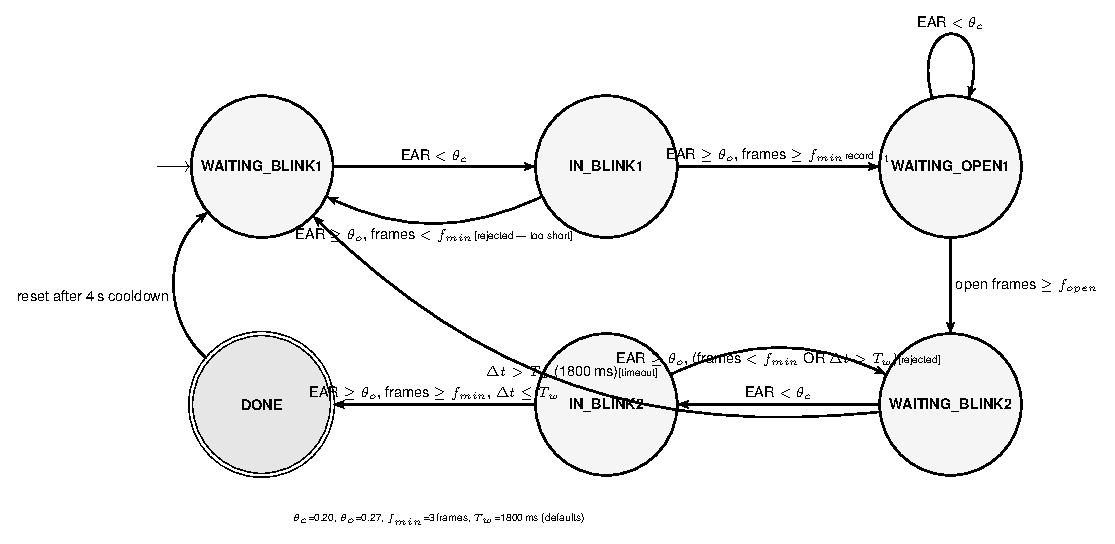
\includegraphics[width=\columnwidth]{../template/figures/fig_statemachine}
  \caption{Máquina de estados de dupla piscada deliberada de seis estados. Transições
    tracejadas indicam caminhos de rejeição que resetam o autômato.
    $\theta_c{=}0{,}20$, $\theta_o{=}0{,}27$, $f_\text{min}{=}3$\,quadros,
    $T_w{=}1800$\,ms.}
  \label{fig:maquinadeestados}
\end{figure}

\subsection{Calibração Específica por Paciente via DetectionProfile}
\label{sec:calibracaopaciente}

As características faciais do paciente variam substancialmente — o EAR de linha de
base depende da abertura palpebral, distância face-câmera e iluminação. O NeuroAssist AI
acomoda isso por meio do \emph{DetectionProfile}: um registro de configuração versionado
e imutável que vincula o conjunto de tipos de gesto ativos (\texttt{TipoGesto}) ao
agente de borda voltado ao paciente.

O campo \texttt{engineFeatureRef} (e.g., \texttt{"mp.blink.double.v1"}) é um token de
string que identifica qual algoritmo de detecção o agente de borda deve ativar para cada
primitiva. Esse desacoplamento significa que adicionar um novo tipo de gesto — como um
detector de aceno de cabeça ou pressão labial — requer registrar um novo
\texttt{TipoGesto} com um novo \texttt{engineFeatureRef} sem modificar nenhum código
de domínio existente.

\subsection{Arquitetura de Microsserviços Hexagonal}
\label{sec:hexagonal}

Cada microsserviço (\texttt{gest-service}, \texttt{evnt-service}) é estruturado de
acordo com a arquitetura de Portas e Adaptadores (hexagonal)~\cite{cockburn2005hexagonal},
aplicada pelo ArchUnit~\cite{archunit} em tempo de compilação. Nove regras de
arquitetura são aplicadas a cada build (Tabela~\ref{tab:archunit}). As regras
\textsc{rule-01} e \textsc{rule-02} garantem que a camada de domínio não tenha
importações de framework, tornando a lógica de negócio central testável de forma
independente. \textsc{Rule-03} impede que o gerenciamento de transações vaze para
controladores ou adaptadores.

\begin{table}[htbp]
\centering
\caption{Regras de aplicação ArchUnit (em tempo de compilação).}
\label{tab:archunit}
\begin{tabular}{ll}
\toprule
Regra & Restrição \\
\midrule
RULE-01 & \texttt{domain.*} não deve importar \texttt{org.springframework} \\
RULE-02 & \texttt{domain.*} não deve importar \texttt{jakarta.persistence} \\
RULE-03 & \texttt{@Transactional} somente em \texttt{application.service} \\
RULE-04 & \texttt{api.*} não deve depender de \texttt{infrastructure.*} \\
RULE-05 & \texttt{infrastructure.*} não deve depender de \texttt{api.*} \\
RULE-06 & \texttt{@FeignClient} somente em \texttt{infrastructure.clients} \\
RULE-07 & Sem injeção de campo \texttt{@Autowired} \\
RULE-08 & \texttt{spring.jpa.open-in-view=false} obrigatório \\
RULE-09 & Pacote base deve ser \texttt{com.neuroassist.<module>} \\
\bottomrule
\end{tabular}
\end{table}

\subsection{Pipeline de Ingestão de Eventos em Doze Etapas}
\label{sec:ingestao}

O recebimento de um relatório de gesto do agente de borda aciona um pipeline
transacional de doze etapas no \texttt{ReportIngressService}: (1)~verificação de
idempotência via \texttt{reportId} UUID; (2)~validação do gesto contra o perfil de
detecção ativo; (3)~snapshot do comando; (4)~roteamento do cuidador; (5)~criação do
\texttt{Evento} com timestamp \texttt{createdAt} do servidor e \texttt{recognizedAt}
do dispositivo; (6)~criação do \texttt{NotificationDispatch} com tier
\texttt{FULL\_SCREEN\_ALARM}; (7--9)~persistência atômica do evento, despacho e
chave de idempotência em uma única fronteira \texttt{@Transactional}; (10)~invocação
do despacho de notificação; (11)~trilha de auditoria; (12)~resposta HTTP\,201 ao
agente de borda.

\subsection{Escopo do PoC e Fronteiras Arquiteturais}
\label{sec:escopopoC}

A Tabela~\ref{tab:escopo} distingue os componentes avaliados neste trabalho daqueles
presentes na arquitetura completa, mas fora do escopo deste artigo.\footnote{Os eventos
de alarme confirmados por gesto produzidos pelo pipeline do NeuroAssist AI são
estruturalmente compatíveis com os formatos de timestamp de eventos utilizados em
pesquisas de monitoramento de VNI~\cite{stell2024pva, yang2026pva}, sugerindo um
caminho de integração futuro no qual eventos de angústia sejam correlacionados com
fluxos de dados do ventilador.} O PoC exclui intencionalmente multilocação,
autenticação e mensageria assíncrona a fim de isolar e validar a latência ponta-a-ponta
gesto-para-alarme e o comportamento de falsos positivos.

\begin{table}[htbp]
\centering
\caption{Componentes implementados vs.\ stub/planejados na avaliação do PoC.}
\label{tab:escopo}
\begin{tabular}{p{3.8cm}p{3.8cm}}
\toprule
\textbf{Implementado (avaliado)} & \textbf{Stub ou trabalho futuro} \\
\midrule
Detecção MediaPipe WASM & Push notifications (FCM/APNs) \\
Máquina de estados de 6 estados & SSE (substitui polling) \\
Versionamento DetectionProfile & Serviço PAC (catálogo) \\
Pipeline de ingestão 12 etapas & Serviço HIST (auditoria) \\
Idempotência via \texttt{reportId} & Serviço ACS (cuidadores) \\
Alarme Angular tela cheia & JWT / OAuth2 \\
Fluxo de confirmação do cuidador & JMS / ActiveMQ Artemis \\
                                 & EDGE (onboarding de dispositivo) \\
\bottomrule
\end{tabular}
\end{table}
